%\chapter{System Architecture}
\chapter{Proposed Methodology}
\label{System Architecture}



\section{Introduction}

{\color{blue}\textbf{Purpose:}
Provide an overview of what the chapter covers — the conceptual structure of your study, theoretical foundations, and the system or model architecture.} \\

{\color{red}\textbf{Writing Instructions:}
\begin{enumerate}
    \item Start with a short paragraph linking from Chapter 2: ``Building on the insights gained from the literature review, this chapter develops the conceptual and system framework underlying the study.''
    
    \item Explain the structure of the chapter: what frameworks, models, or methodologies will be presented.
    
    \item Mention the logical flow — from theoretical conception to system design or implementation approach.
\end{enumerate}}




\section{Conceptual Framework}

{\color{blue}\textbf{Purpose:}
Define and explain the conceptual or theoretical model that guides your study. This framework demonstrates how variables, processes, or modules interact to solve your research problem.} \\

{\color{red}\textbf{Writing Instructions:}
\begin{enumerate}
    \item Begin with a definition of what your conceptual framework represents (e.g., theoretical model, workflow, system process, or hypothesis network).
    
    \item Include a diagram (Figure 3.1) that visually represents the framework.
    
    \item Use labeled boxes and arrows to show relationships or data flow.
    
    \item Follow IEEE figure formatting (caption below, sentence case).
    
    \item Describe each component of the diagram in clear, numbered paragraphs.
    
    \item Explain the purpose, relationship, and expected function of each part.
    
    \item Justify your framework design based on literature (refer back to Chapter 2).
    
    \item End with a summary linking how this conceptual model will guide system design or methodology in later sections.
\end{enumerate}}

\section{System Architecture}

{\color{blue}\textbf{Purpose:}
Translate the conceptual framework into a technical or methodological architecture — the practical structure of your research system, model, or experimental setup.} \\

{\color{red}\textbf{Writing Instructions:}
\begin{enumerate}
    \item Begin with a paragraph summarizing the general system design approach — what kind of architecture is used (layered, modular, client–server, pipeline, etc.).
    
    \item Present a system architecture diagram (Figure 3.2).
    
    \item Describe each system component (software modules, data sources, processing units).
    
    \item Explain how these components interact to fulfill research objectives.
    
    \item Include methodology flow if this involves experimental research (input → process → output).
    
    \item Reference tools and techniques briefly (details will appear in implementation or Chapter 4).
\end{enumerate}


\textbf{Instruction:} Methodology refers to the systematic and structured approach used in a research study to gather, analyze, and interpret data. It outlines the specific procedures, techniques, and tools employed to address the research questions or objectives. A well-defined methodology provides a clear roadmap for the research process, ensuring the reliability and validity of the study. This section typically includes details on the research design, sampling methods, data collection techniques, and data analysis procedures. The methodology allows other researchers to replicate the study and assess its rigor. It plays a critical role in establishing the credibility of research findings and is essential for drawing meaningful conclusions from the collected data. }



\begin{figure}[ht]
    \centering
    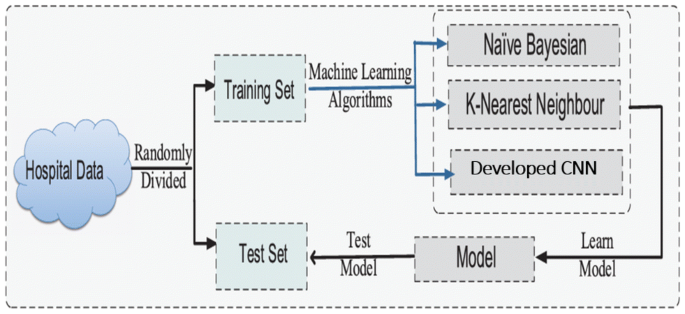
\includegraphics[width=0.90\textwidth]{Images/ML pipeline for detection task on medical imaging data.png}
    \caption{A ML pipeline for detection task on medical imaging data.}
    \label{fig:mlpipeline1}
\end{figure}


\subsection{Algorithms and Model Explanation}

{\color{blue}\textbf{Purpose:}
Describe the computational or logical methods used in your research — algorithms, formulas, or models that underpin your system.} \\

{\color{red}\textbf{Writing Instructions:}
\begin{enumerate}
    \item Write algorithm steps in numbered pseudocode format (use Algorithm environment in LaTeX).
    
    \item Include any mathematical equations (clearly numbered as Eq. 3.1, Eq. 3.2).
    
    \item Explain the logic of your model — how inputs are transformed into outputs.
    
    \item Describe parameter settings, training process (if ML model), or logical flow.
    
    \item Provide a complexity or performance analysis if applicable (Big-O, time, memory, etc.).
\end{enumerate}}


\subsection{Data Flow Diagram (if applicable)}

{\color{blue}\textbf{Purpose:}
Illustrate how data moves within the system — from input to storage, processing, and output.}

{\color{red}\textbf{Writing Instructions:}
\begin{enumerate}
    \item Use standard DFD notations (process, data store, data flow, external entity).
    
    \item Present Level-0 (context) and Level-1 diagrams if your system is complex.
    
    \item Label all entities and flows clearly.
    
    \item Describe each process in 1–2 sentences under the figure.
    
    \item Ensure the diagram corresponds exactly to the modules described earlier.
\end{enumerate}


\begin{itemize}
    \item Describe the research design, methods, and procedures used in your project/thesis.
    \item Explain the data collection/requirement identification and analysis techniques.
    \item Discuss any ethical considerations and limitations of your study.
\end{itemize}}



\section{Data Collection Process and Analysis}

{\color{blue}\textbf{Purpose:}
Explain how data is collected, processed, and analyzed in your study — bridging design with analytical methodology.} \\

{\color{red}\textbf{Writing Instructions:}
\begin{enumerate}
    \item Start by explaining your data flow process (collection → preprocessing → analysis).
    
    \item Justify the choice of data source — show reliability and relevance.
    
    \item Explain data preparation steps (cleaning, normalization, feature extraction).
    
    \item Describe analysis techniques — statistical, computational, or experimental.
    
    \item Present sample formats, variables, or data schema diagrams if applicable.
    
    \item Mention tools or software used for analysis (e.g., Python, MATLAB, R).
\end{enumerate}


Data presentation and analysis constitute a pivotal phase in the research process, where collected information is organized, interpreted, and communicated effectively. In this stage, raw data are transformed into meaningful insights through various statistical or qualitative methods, depending on the research design. Data presentation involves visually representing the findings using tables, charts, graphs, or other visual aids to enhance clarity and comprehension. Analysis, on the other hand, encompasses the systematic examination of the data to uncover patterns, relationships, and trends. This process not only validates the research outcomes but also enables researchers to draw meaningful conclusions and make informed interpretations. Effectively presenting and analyzing data is essential for conveying the significance of the research findings to both academic and non-academic audiences. 

\begin{itemize}
    \item Present the data collected during your project.
    \item Use tables, graphs, charts, or other visuals to enhance clarity.
    \item Analyze the data and draw conclusions based on your findings.
\end{itemize} }




\subsection{ Data Collection Methods}

{\color{blue}\textbf{Purpose:}
Document the techniques used to gather information, datasets, or experimental measurements.} \\

{\color{red}\textbf{Writing Instructions:}
\begin{enumerate}
    \item State clearly what type of data (primary, secondary, simulated, experimental).
    
    \item Describe the instruments, sources, or platforms used (surveys, sensors, APIs, etc.).
    
    \item Explain data validation (quality control, filtering, calibration).
    
    \item If using human participants, note ethical approval and consent.
\end{enumerate}}

\subsection{Data Analysis Techniques}

{\color{blue}\textbf{Purpose:}
Explain how raw data is transformed into meaningful information.}

{\color{red}\textbf{Writing Instructions:}
\begin{enumerate}
    \item Describe statistical, computational, or analytical techniques used (e.g., regression, clustering, hypothesis testing, evaluation metrics).
    
    \item Justify why each method was chosen.
    
    \item Present formulae, tools, or frameworks used.
    
    \item Discuss limitations or assumptions (normality, independence, etc.).
\end{enumerate}}

\section{Engineering and Societal Considerations}
{\color{blue}\textbf{Purpose:}
Demonstrate professional responsibility — that your design or system adheres to ethical, environmental, and social standards.} \\

{\color{red}\textbf{Writing Instructions:}
\begin{enumerate}
    \item Introduce the idea that technical innovation must align with engineering ethics and sustainability.
    
    \item Divide into three key subsections: societal impact, environmental considerations, and ethical responsibility.
    
    \item Use real examples (e.g., carbon footprint, accessibility, data privacy).
    
    \item Link your considerations to relevant global frameworks (IEEE Code of Ethics, SDGs, GDPR).
\end{enumerate}

Engineering considerations encompass a set of crucial factors that engineers must weigh during the design, development, and implementation of projects.}

\subsection{Societal Impacts of Engineering Solutions}

{\color{blue}\textbf{Purpose:}
Evaluate how your system affects people, communities, or industries.} \\

{\color{red}\textbf{Writing Instructions:}
\begin{enumerate}
    \item Discuss both positive outcomes (efficiency, inclusion) and potential negative effects (job displacement, privacy risks).
    
    \item Relate to real-world case studies or applications.
    
    \item Emphasize alignment with human-centered design principles.
\end{enumerate}

The relationship between the engineer and society involves recognizing the societal impacts of engineering solutions, including considerations for safety, accessibility, and the overall well-being of communities. Engineers are increasingly mindful of their role in promoting social responsibility and addressing diverse needs.}

\subsection{Environment and Sustainability Considerations}

{\color{blue}\textbf{Purpose:}
Assess your system’s environmental footprint and contribution to sustainability.} \\

{\color{red}\textbf{Writing Instructions:}
\begin{enumerate}
    \item Discuss energy efficiency, hardware usage, or green data practices.
    
    \item Show how your work supports one or more UN Sustainable Development Goals (SDGs).
    
    \item Mention design decisions that reduce resource use or waste.
\end{enumerate}

Environment and sustainability considerations involve assessing and mitigating the environmental impact of engineering projects. This includes minimizing resource depletion, reducing pollution, and promoting sustainable practices to ensure long-term ecological balance. Sustainable engineering aims to create solutions that meet present needs without compromising the ability of future generations to meet their own needs.}

\subsection{Ethical and Professional Responsibility}

{\color{blue}\textbf{Purpose:}
Show compliance with ethical standards and academic integrity.} \\

{\color{red}\textbf{Writing Instructions:}
\begin{enumerate}
    \item Reference professional codes (IEEE, ACM, ISO, Belmont Report).
    
    \item Mention data privacy, informed consent, plagiarism avoidance, and responsible AI (if relevant).
    
    \item Include institutional approval if human data are used.
\end{enumerate}
Ethics in engineering emphasizes the moral and professional responsibilities of engineers. Ethical considerations involve ensuring the safety, honesty, and integrity of engineering practices. Engineers are expected to prioritize the well-being of individuals and communities, uphold transparency, and adhere to ethical codes in their decision-making processes.}
